\section{Selection Efficiency and Outreach Information}
\label{sec:seleff}
We would like to quote our results as a cross-section, or cross-section limit, that is as
model independent as possible. 
For this we carefully define the acceptance, and provide enough
details about the selection efficiency within that acceptance that anybody can use their favorite Monte Carlo
generator of new physics, define an acceptance at the hard scatter level (status = 3 in Pythia), and correctly estimate
the efficiency for this new physics model to within 50\% or so (the so-called
``outreach'' program).
The same steps are done here as in the pre-tagged sample analysis~\cite{ssnote2011}
with appropriate modifications considering differences in selections of leptons
and an addition of the $b$-tagged jet requirements.

The event selection efficiency is a combination of 
\begin{enumerate}
\item the kinematical requirements on leptons and jets
\item the lepton identification and isolation efficiency;
\item the efficiency of the \met\ requirement;
\item the efficiency of the \Ht\ requirement;
\item the efficiency of the $b$-jet tagging requirement.
\end{enumerate}
We derive efficiency functions for 
components 2 to 5 using a sample of simulated events
for the LM6 SUSY model point.\footnote{The LM6 cMSSM model point 
is defined by the model parameters as $m_0 = 85~\GeV$, $m_{1/2} = 400~\GeV$, $\tan\beta = 10$, $\mu>0$,
and $A_0 = 0~\GeV$.}
Applicable simulation-to-data corrections (scale factors) are also evaluated based on 
available comparisons of these effiencies in data and simulation.
As described below, the description of the lepton selections
does not require an additional scale factor,
and the correction for $b$-tagged jets is small with a scale factor of 0.96.

\subsection{Definition of Acceptance}
\label{sec:acceptance}
%
Lepton acceptance is defined for both leptons with $|\eta|<2.4$ and $\pt > 20~\GeV$.
The generator-level equivalent of the \Ht, $\Ht^{\rm gen}$, is comprised of the sum $\pt$ of all colored particles 
at the hard scatter level that have $\pt > 40$ GeV and $|\eta |<2.5$.
The number of such colored particles defines the number of jets at generator
level. 
A generator-level \met\ equivalent, $\met^{\rm~gen}$, is defined as the absolute value of the vector sum of the transverse 
momentum of all non-interacting particles, e.g. neutrinos and LSP.
%
%
\subsection{Lepton Efficiencies}
\label{sec:lepeff}
%
The electon and muon selection efficiency dependence as a function of the lepton \pt\
is shown in Fig.~\ref{fig:lepeffLM6}.
It is derived using LM6 events passing the baseline selections applied to jets and a \met~$>$ 30 \GeV~requirement.
Compared to the pre-tagged sample analysis~\cite{ssnote2011}, we obtain a slightly
lower efficiency, consistent with the tighter requirement on isolation.

\begin{figure}[h]
\begin{center}
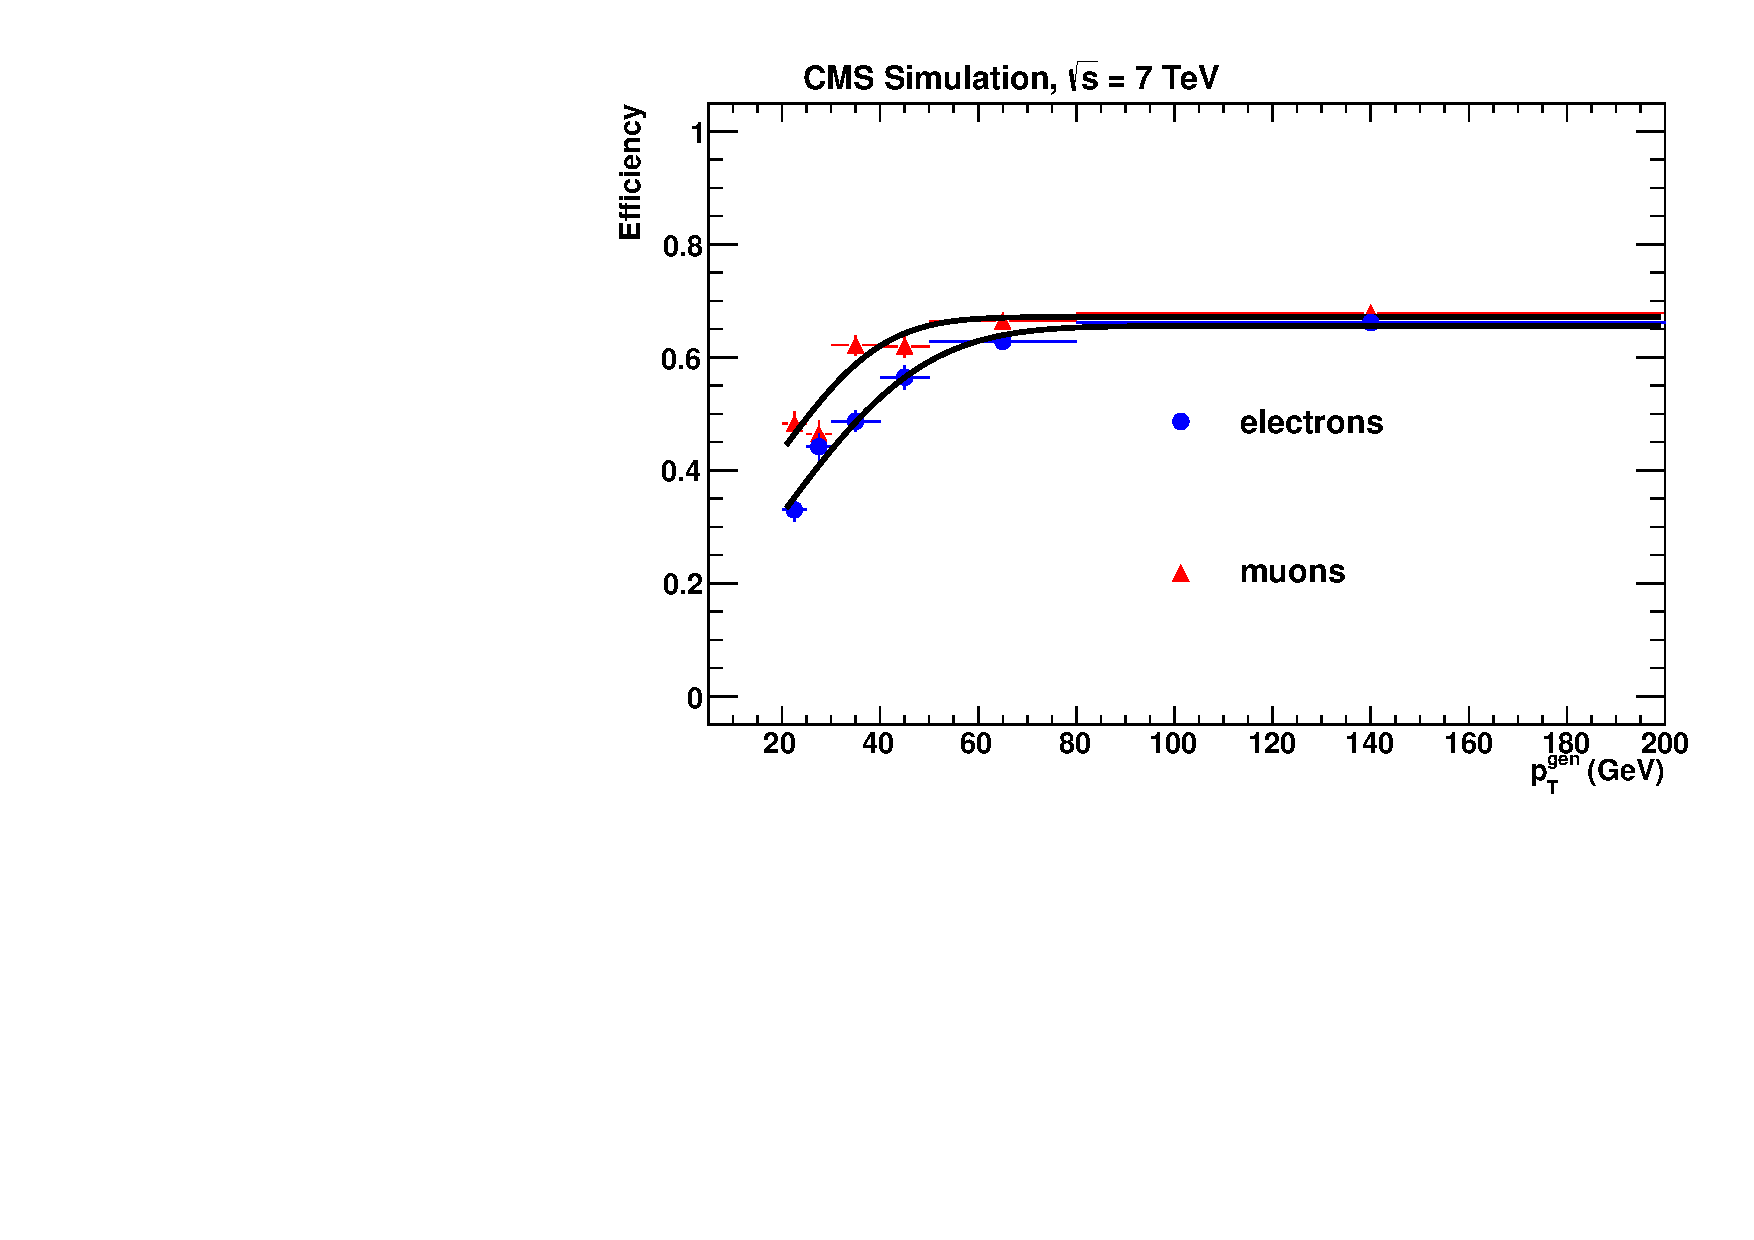
\includegraphics[width=0.7\linewidth]{figs/leptonEfficiency_lm6}
\caption{\label{fig:lepeffLM6}
Lepton selection efficiency as a function of \pt,
displayed for electrons and muons.
}
\end{center}
\end{figure}

%
The efficiency dependence can be parameterzied as a function of \pt\ as 
%
\begin{eqnarray}
\epsilon = \epsilon_{\rm \infty} {\rm erf}\left ( \frac{\pt - C}{\sigma} \right)
	+ \epsilon_C \left( 1.- {\rm erf}\left ( \frac{\pt - C}{\sigma} \right) \right),
\label{eq:lepeffFitF}
\end{eqnarray}
where $\epsilon_{\rm \infty}$ gives the value of the efficiency plateau at high momenta,
$C$ is equal to 20~\GeV,
$\epsilon_C$ gives the value of the efficiency at $\pt=C$,
and $\sigma$ describes how fast the transition region is.
The results of the fit for electrons and muons are summarized in Table~\ref{tab:lepeffLM6fit}.
%
\begin{table}[h]
\begin{center}
\caption{\label{tab:lepeffLM6fit} Results of the fit of the dependence in Fig.~\ref{fig:lepeffLM6}
to the function specified in Eq.~\ref{eq:lepeffFitF}.}
\begin{tabular}{l|cc}\hline\hline
Parameter		& Electrons		& Muons			\\ \hline
$\epsilon_{\infty}$	& 0.656	& 0.672	\\
$\epsilon_{C}$		& 0.322	& 0.435	\\
$\sigma$		& 32.3  & 22.9	\\
\hline\hline
\end{tabular}
\end{center}
\end{table}

%
%
\subsection{Trigger Efficiency}
\label{sec:trg}
As discussed in Section~\ref{sec:eventsel}, this analysis uses dilepton
triggers; the lepton $p_{T}$ thresholds are high enough that we do 
not need the dilepton$+ H_T$ triggers.  The trigger efficiency, as 
discussed in Reference~\cite{ssnote2011}, is $99 \pm 1\%$ 
($96 \pm 3\%$) per electron (muon).


\subsection{\met\ and $\Ht$ efficiency turn-on}
\label{sec:turnon}
Our selections on reconstructed jets begin with a requirement of at least two jets with $\pt>40~\GeV$.
%Two such jets are present in approximately 95\% 
% of the events in LM1 and LM6 with $\Ht^{\rm gen}>200~\GeV$ prior
%to any additional requirement on colored partons at the generator 
% level beyond the sum of \pt.
%This represents the fraction of acceptance to two jets.
In the following we proceed with determining $\Ht$ and \met\ requirements with respect to 
events that have generator-level requirements on the leptons and colored particles as described in Section~\ref{sec:acceptance}.
%
The efficiency for an event to pass a given reconstructed \met\ ($\Ht$) threshold is shown in Fig.~\ref{fig:htmetThresh}
as a function of $\met^{\rm~gen}$ ($\Ht^{\rm gen}$) in events passing $\Ht^{\rm gen}>200~\GeV$ ($\met^{\rm~gen}>30~\GeV$).
Due to the rather small fraction of events in LM6 simulation having low \Ht\ activity, the \Ht\ curves are made with LM1.\footnote{The LM1 cMSSM model point 
is defined by the model parameters as $m_0 = 60~\GeV$, $m_{1/2} = 250~\GeV$, $\tan\beta = 10$, $\mu>0$,
and $A_0 = 0~\GeV$.}
Results of the fits of these curves to $0.5 \epsilon_{\infty} \{{\rm erf}[(x - x_{1/2})/\sigma] + 1\}$ are summarized
in Table~\ref{tab:htmetThresh}.
Neither the \met\ nor \Ht\ curves show a significant bias in the position of the point with half the plateau efficiency ($x_{1/2}$).
The inefficiency at the plateau is essentially negligible.
The width of the threshold $\sigma$ increases with the value of the cut.
%
\begin{figure}[h]
\begin{center}
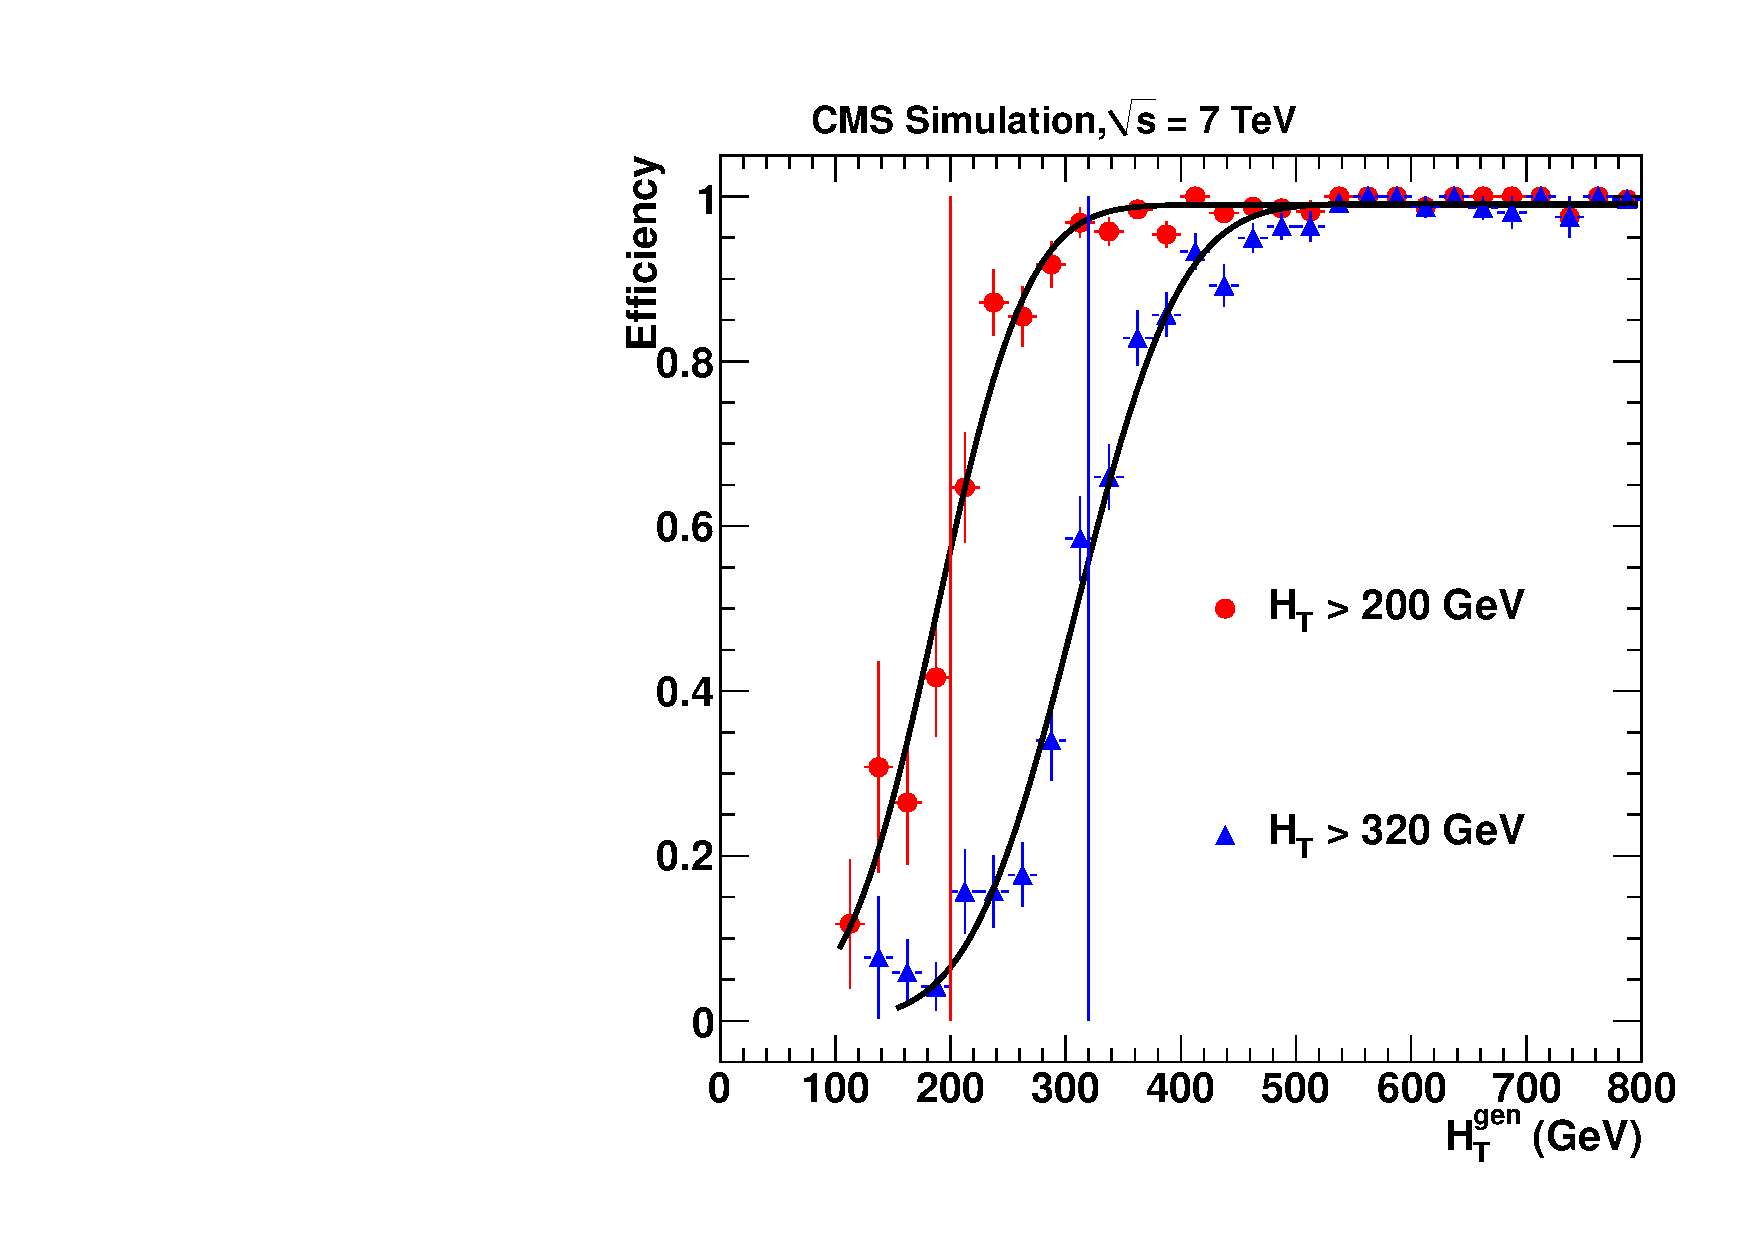
\includegraphics[width=0.48\linewidth]{figs/HTturnOnCurve_lm1}
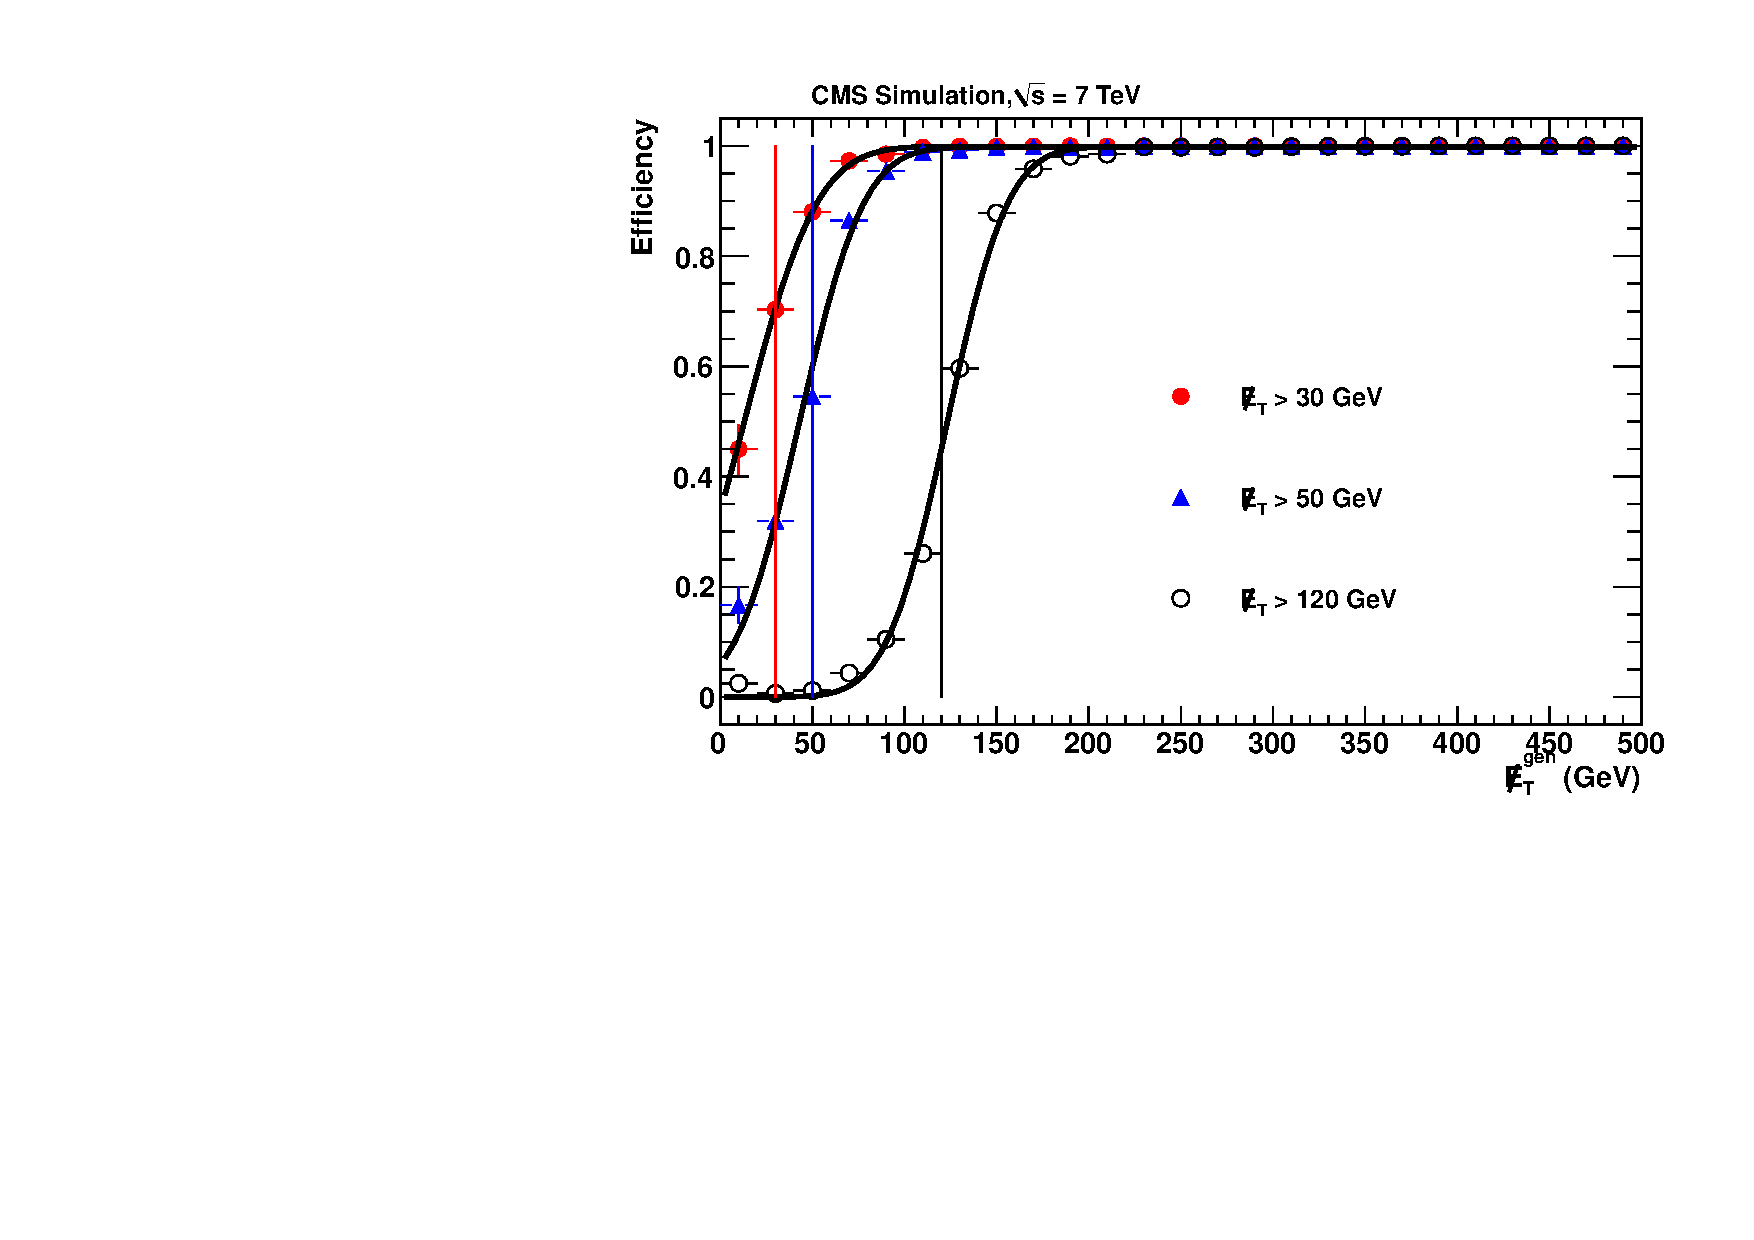
\includegraphics[width=0.48\linewidth]{figs/metTurnOnCurve_lm6}
\caption{\label{fig:htmetThresh}
Efficiency for an event to pass a given reconstructed \met\ ($\Ht$) threshold 
as a function of $\met^{\rm~gen}$ ($\Ht^{\rm gen}$).
The curves are shown for \met\ thresholds of 30, 50, and 120~\GeV;
the thresholds for \Ht\ are 200, 320~\GeV.
}
\end{center}
\end{figure}
%
%
\begin{table}[h]
\begin{center}
\caption{\label{tab:htmetThresh} Results of the fit of the dependence in Fig.~\ref{fig:htmetThresh}
to $0.5 \epsilon_{\infty} \{{\rm erf}[(x - x_{1/2})/\sigma] + 1\}$.}
\begin{tabular}{l|cc|ccc}\hline\hline
Parameter		& \multicolumn{2}{|c}{\Ht}			& \multicolumn{3}{|c}{\met}			\\ 
			&	$>200~\GeV$	&	$>320~\GeV$		& $>30~\GeV$		& $>50~\GeV$		& $>120~\GeV$	\\ \hline
$\epsilon_{\infty}$	& $0.990\pm0.002$	& $0.992\pm0.003$	& $0.999\pm0.001$	& $0.999\pm0.001$	& $0.999\pm0.001$ \\
$x_{1/2}$,~\GeV		& $187.8\pm 5.5$	& $308.4\pm 3.3$		& $13.1\pm2.4$		& $43.0\pm1.1$		& $123.3\pm 0.5$  \\
$\sigma$,~\GeV		& $88.3\pm9.8$		& $102.0\pm6.2$		& $44.0\pm2.8$		& $38.9\pm1.6$		& $36.6\pm0.9$	\\
\hline\hline
\end{tabular}
\end{center}
\end{table}


\subsection{Jet $b$-tagging efficiency}
\label{sec:btagEff}
The $b$-jet tagging efficiency is defined for b-quarks passing $|\eta|< 2.5$ and matching to a reconstructed jet.
A fraction of these b-quark that match to a b-tagged jet is the b-jet tagging efficiency.
It shown in Fig.~\ref{fig:btagEff} as a function of the b-quark \pt.
For b-quarks of $|\eta| < 2.5$, the b-jet tagging efficiency as a function 
of \pt~can be parametrized as 
%\begin{itemize}
%\item \pt~ $<$~ 90 GeV:~~~~~~~~~~~~~~~~$\epsilon = SF \cdot [p0 \cdot (p_t-90~{\rm GeV}) + p1]$
%\item 90 GeV $<$~ \pt$~ <$ 170 GeV:~~~~$\epsilon = SF \cdot p1$
%\item \pt~ $>$ 170 GeV:~~~~~~~~~~~~~~$\epsilon = SF \cdot [p2 \cdot (p_t-170~{\rm GeV}) + p1]$
%\end{itemize}

\begin{table}[!h]
\begin{center}
\begin{tabular}{@{\textbullet}ll}
	~~$p_{T } >$ 90 GeV &  $\epsilon = SF \cdot [p_{0} \cdot (p_{T} - 90~{\rm GeV}) + p_{1}]$ \\
	~~90 GeV $< p_{T} <$ 170 GeV & $\epsilon = SF \cdot p_{1}$ \\
	~~$p_{T} >$ 170 GeV & $\epsilon = SF \cdot [p_{2} \cdot (p_{T} - 170~{\rm GeV}) + p_{1}]$ \\
\end{tabular}
\end{center}
\end{table}

\noindent where the parameters $p_{0}$, $p_{1}$, and $p_{2}$ are given in Figure~\ref{fig:btagEff}
and $SF$ is the data-Monte Carlo scale factor: $SF$ = 0.96 with a 
4 (15)\% uncertainty for jets with $\pt<240 (>240)~\GeV$ (see 
Section~\ref{sec:bjetSF}). 
% {\bf Make sure that the parametrization is correct.}

\begin{figure}[h]
\begin{center}
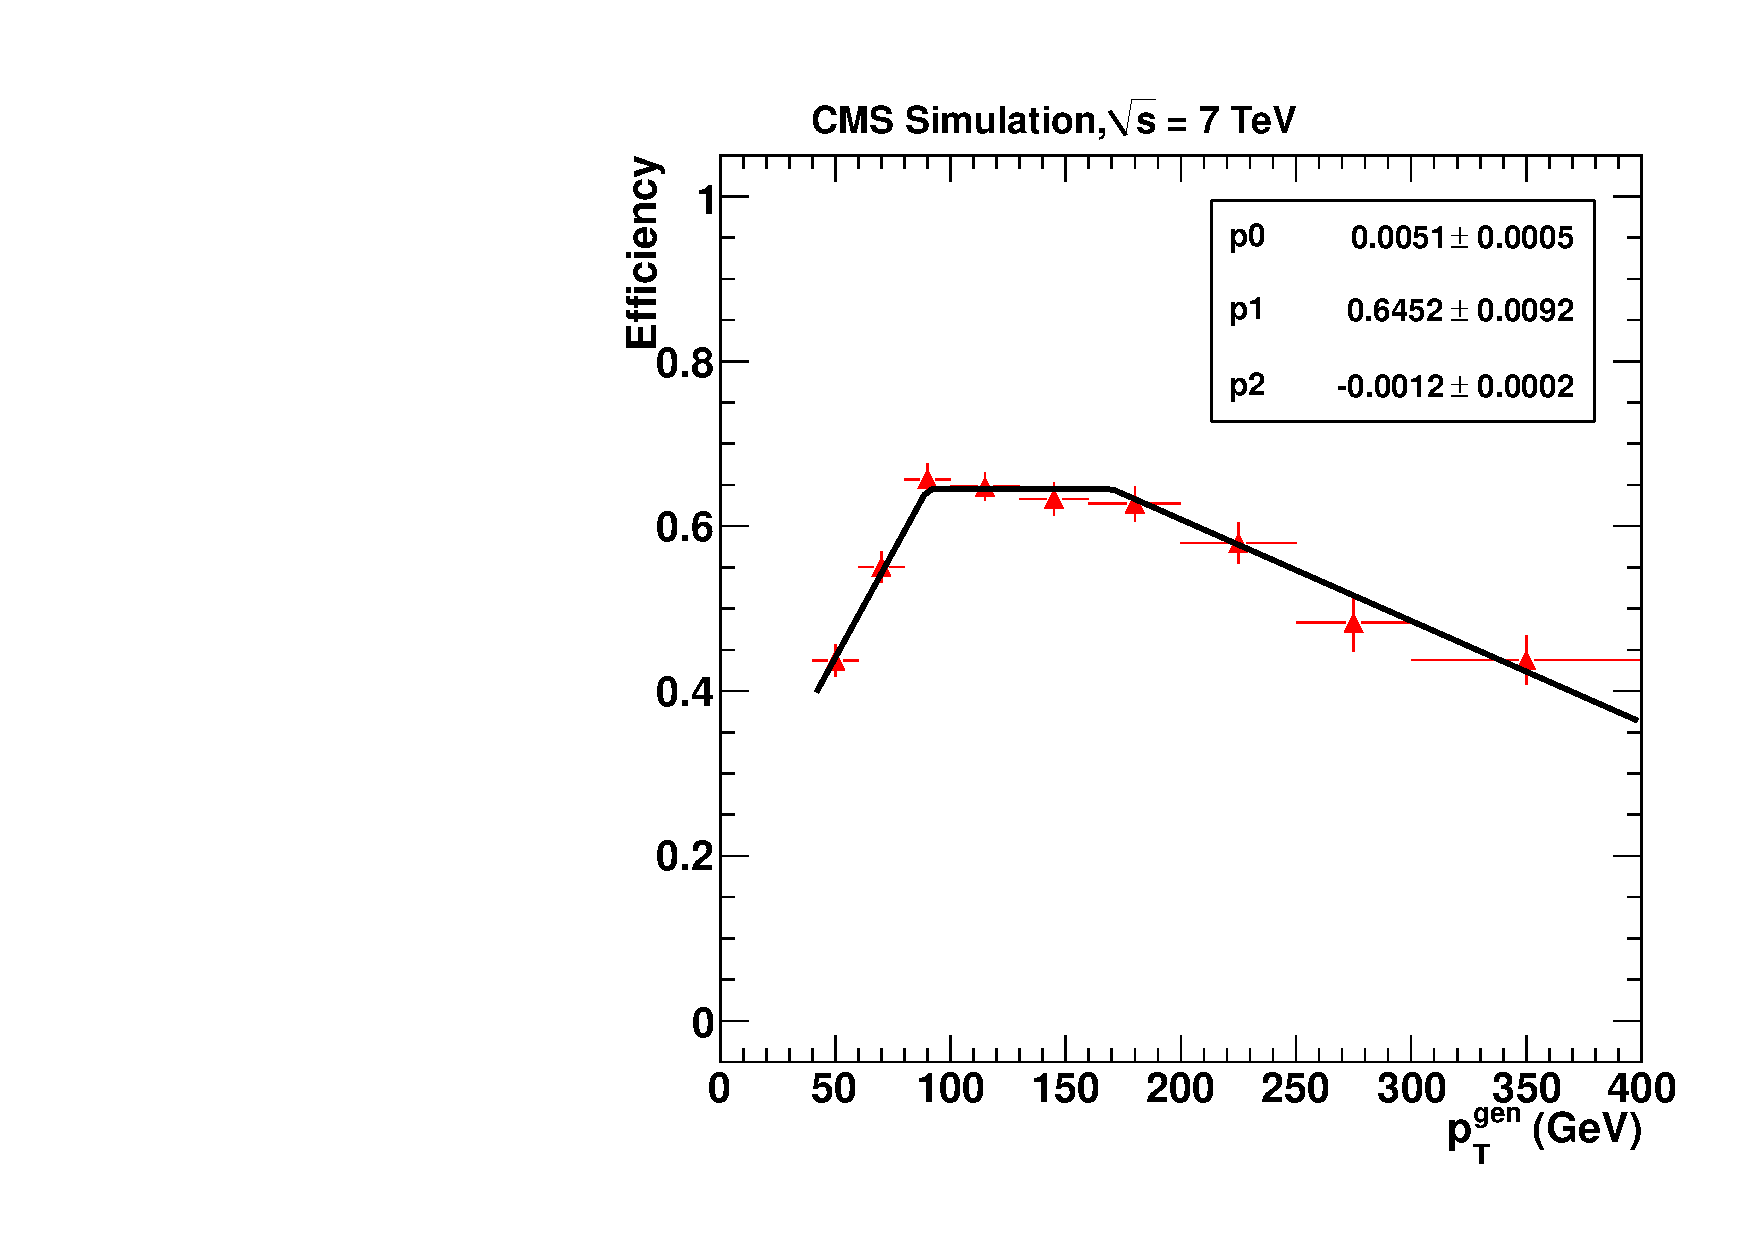
\includegraphics[width=0.48\linewidth]{figs/btagEfficiency_lm6.pdf}
\caption{\label{fig:btagEff}
$B$-jet tagging efficiency as a function of the matching b-quark \pt~ in LM6 SUSY MC.
}
\end{center}
\end{figure}

\subsection{Data - Monte Carlo Scale Factors and their Uncertainties}
\label{sec:SF}

\subsubsection{Data - Monte Carlo Scale Factor for Leptons}
\label{sec:tnp}

The efficiencies of the lepton isolation and identification requirements (including all quality requirements) 
are measured with the tag\&probe method in dilepton Z events using the full 2011 dataset.
The efficiency of the identification requirements is a property of the lepton itself and is directly applicable
 to the leptons in signal events.
The efficiency of the isolation requirement, however, is a strong function of all other (mainly hadronic)
activity in the event.
The following results are based on measurements using the full dataset and compared 
to simulation that is re-weighted to have a pile-up distribution comparable to that observed in data.

The electron selection efficiencies are measured in events passing 
the \verb=Ele17..._SC8_Mass30= and \\\verb=Ele17.._Ele8_Mass30= triggers,
which require one well-identified electron and one super-cluster or GSF electron with $\pt>8~\GeV$ forming a pair with a mass
above 30~\GeVcc.  
For higher $\pt$ electrons, the \verb=Ele32...SC_17= triggers are also used, 
which require one well identified electron and one super-cluster with $\pt >17~\GeV$.
In the tag\&probe analysis the electron tag is required to match to the well-identified electron 
from the trigger and also to pass all the electron requirements described in~\cite{ssnote2011}.
The probe electron is required to have
\begin{itemize}
\item $\pt>20~\GeV$, $|\eta|<2.4$, excluding the super-clusters with $1.4442<|\eta|<1.566$.
\end{itemize}
The isolation efficiency is measured with the probes passing all electron selections, except for the 
trigger requirement and the isolation itself.
The identification efficiency is measured with probes passing the isolation requirement.
Results of the measurement are summarized in Table~\ref{tab:eleEffs}.
The contribution from the Z events is based on simple counting in the mass range of 86--96~\GeVc.  The MC contribution includes W+jets events to match the expected residual backgrounds in this mass window.
The following sources of systematic uncertainty are attributed to this measurement:
background contribution, selection of dielectron events, factorization of the isolation and ID parts.
The size of the background contribution can be estimated using MC alone
and also  tested in data with  the same-sign dielectron
events, which should represent the number of backgrounds reasonably well.
The effect of backgrounds on the measured efficiency is established to be approximately 
2\% for the combined identification
and isolation selection efficiency.
The narrow mass window used to count electron pairs introduces a bias of about 3\% 
to the measured efficiency
by rejecting failing probes that happen to have a worse resolution or a shift
in the measured momentum.
This bias is expected to approximately cancel in data and simulation.
We include a half of the 3\% as a source of systematics.
Based on simulation alone, the combined selection efficiency, measured with respect to the probe electron,
differs from the product of the components by approximately 1\% or less depending on the momentum range.
All of these effects combined give a systematic uncertainty on the total data-to-MC scale factor
in the lepton selection efficiencies of 2.5\% for $\pt>20~\GeV$.

\begin{table}[h]
\begin{center}
\begin{tabular}{c|c|ccc}
\hline\hline
& & 20 - 40 GeV & 40 GeV -  \\
\hline
				& MC			& 	0.9268 $\pm$ 0.0004 & 	0.9768 $\pm$ 0.0002 \\
ISO				& DATA			& 	0.9247 $\pm$ 0.0003 & 	0.9737 $\pm$ 0.0002 \\
				& DATA/MC		& 	0.9977 $\pm$ 0.0005 & 	0.9968 $\pm$ 0.0003 \\
\hline
				& MC			& 	0.8069 $\pm$ 0.0005 & 	0.8500 $\pm$ 0.0004 \\
ID				& DATA			& 	0.8005 $\pm$ 0.0005 & 	0.8343 $\pm$ 0.0004 \\
				& DATA/MC		& 	0.9921 $\pm$ 0.0008 & 	0.9815 $\pm$ 0.0006 \\
\hline
				& MC			& 	0.7478 $\pm$ 0.0005 & 	0.8303 $\pm$ 0.0004 \\
ID X ISO			& DATA			& 	0.7403 $\pm$ 0.0005 & 	0.8124 $\pm$ 0.0004 \\
				& DATA/MC		& 	0.9899 $\pm$ 0.0010 & 	0.9784 $\pm$ 0.0007 \\
\hline \hline
\hline
\end{tabular}
\caption{\label{tab:eleEffs}Electron isolation and identification efficiencies measured with the tag\&probe method.
The uncertainties are statistical only.}
\end{center}
\end{table}

The muon selection efficiencies are measured using events passing the double-muon trigger.
The tag muon is required to pass all of the muon selection requirements described in~\cite{ssnote2011}.
The probe muon is required to pass
\begin{itemize}
\item $\pt>20~\GeVc$;
\item $|\eta|<2.4$;
\item have both the global and the tracker muon types.
\end{itemize}
Both the  isolation and the identification efficiency are measured using probes failing only the requirement in question,
assuming the efficiencies factorize.
Results of the muon identification and isolation efficiency measurements are presented in Table~\ref{tab:muEffs}.
As expected, the identification efficiency for muons measured in data and in MC agree well,
while there is some discrepancy for the isolation efficiency.
Similar sources of systematic uncertainty are considered here as those considered for electrons.
Most of the reconstructed (probe) muons are real muons and the measurement of the identification efficiency
is not affected significantly by backgrounds.
With the tighter mass window used here to select events,
 the backgrounds are estimated to be small.
This narrow mass window, however, introduces a bias of about 1.5\% 
to the measured efficiency
by rejecting failing probes that happen to have a worse resolution or a shift
in the measured momentum.
This bias is expected to approximately cancel in data and simulation.
We include a half of the 1.5\% as a source of systematics.
We assign a systematic uncertainty of 1\% on the identification and isolation efficiency measurement  
from a comparison between the simple counting of Z events and fitting the mass shape to a gaussian signal and an 
exponential background component.
Based on studies in MC events, we find that the isolation and the identification efficiencies
 factorize near-perfectly and do not assign any additional systematic uncertainty.
The total systematic uncertainty on the muon efficiency measurement in 
data, simply covering the full momentum range, is 2\%.


\begin{table}[h]
\begin{center}
\begin{tabular}{c|c|cc}
\hline\hline
& & 20 - 40 GeV & 40 GeV -  \\ 
\hline
				& MC			& 	0.9111 $\pm$ 0.0003& 	0.9747 $\pm$ 0.0002 \\
ISO				& DATA			& 	0.8969 $\pm$ 0.0003& 	0.9668 $\pm$ 0.0002 \\
				& DATA/MC		& 	0.9844 $\pm$ 0.0004& 	0.9919 $\pm$ 0.0002 \\
\hline
				& MC			& 	0.9710 $\pm$ 0.0002& 	0.9612 $\pm$ 0.0002 \\
ID				& DATA			& 	0.9666 $\pm$ 0.0002& 	0.9561 $\pm$ 0.0002 \\
				& DATA/MC		& 	0.9955 $\pm$ 0.0003& 	0.9947 $\pm$ 0.0003 \\
\hline
				& MC			& 	0.8847 $\pm$ 0.0003& 	0.9369 $\pm$ 0.0002 \\
ID X ISO			& DATA			& 	0.8669 $\pm$ 0.0003& 	0.9244 $\pm$ 0.0002 \\
				& DATA/MC		& 	0.9799 $\pm$ 0.0005& 	0.9866 $\pm$ 0.0003 \\
\hline \hline
\end{tabular}
\caption{\label{tab:muEffs}Muon isolation and identification efficiencies measured with the tag\&probe method.
The uncertainties are statistical only.}
\end{center}
\end{table}

The tag\&probe results in Tables~\ref{tab:eleEffs} and~\ref{tab:muEffs}
show that for leptons with $\pt>20~\GeV$ used in this analysis both the ID part and the isolation parts
 of the lepton selection are reproduced well by simulation, already within the systematic uncertainties
quoted above.
Application of this measurement based on Z events to the signal events incurs
an additional uncertainty due to potential mismodeling of the isolation requirement.
In agreement with Ref.~\cite{ssnote2011}, we assign a systematic uncertainty of 5\% 
due to modeling of the isolation efficiency for signal events.
Considering the small size of the difference between data and simulation reported in 
Tables~\ref{tab:eleEffs} and~\ref{tab:muEffs}, compared to the systematic uncertainty
applicable to the analysis,
we approximate the scale factor to be 1.0 for both simulated signal and backgrounds
and propagate the uncertainty described above to the relevant part of the analysis
(signal selections) described in Section~\ref{sec:systematic}.

\subsubsection{Data - Monte Carlo Scale Factor for b-jets}
\label{sec:bjetSF}
We apply an average scale factor of 0.96 measured using \ttbar\ events
for the SSVHEM tagger~\cite{BTV11003}.
The uncertainty on the scale factor is 4 (15)\% for jets with $\pt<240 (>240)~\GeV$,
as recommended by the $b$-tagging POG~\cite{btvSyst}. We apply
it to the analysis as described in Section~\ref{sec:systematic}.
